\documentclass[11pt,a4paper]{article}
\usepackage{graphicx}
\usepackage{amsmath}
\usepackage{geometry}
\geometry{margin=1in}
\graphicspath{{../}}

\title{Assignment 5: Eulerian Two-Fluid Simulations of Fluidized Bed}
\author{Sajeev}
\date{October 2025}

\begin{document}
\maketitle

\section{Eulerian Two-Fluid Model \& KTGF}
The gas-solid fluidization was modeled using the Eulerian Two-Fluid approach. The gas is the primary phase and solid beads are the secondary phase. The governing equations solve mass and momentum conservation for both phases, coupled via interphase exchange terms (Gidaspow drag model).
The Kinetic Theory of Granular Flow (KTGF) was employed to model the solid phase stresses. The granular temperature $\Theta_s$, representing the kinetic energy of random particle fluctuations, is solved via a conservation equation accounting for generation, diffusion, and collisional dissipation.

\section{Simulation Setup}
A pseudo-2D domain ($0.2\times1\times0.02$ m) was meshed uniformly ($20\times70\times4$). Air was injected from the bottom at superficial velocities of $1.736$ m/s and $2.78$ m/s into an initial solid bed height of $0.2$ m ($\alpha_s=0.6$). The Phase-Coupled SIMPLE and 2nd Order Implicit schemes were utilized.

\section{Fluidization Dynamics Analysis}
The simulations capture the transient bubbling dynamics inherent to fluidized beds.
\begin{itemize}
    \item \textbf{Solid Volume Fraction:} At $1.736$ m/s, bubbles are distinct, smaller, and rise uniformly. At $2.78$ m/s, the bubbling is far more vigorous, with larger, coalescing bubbles causing substantial bed expansion and violent surface eruptions.
    \item \textbf{Solid Velocity:} Particles are drawn upward in the bubble wakes and recirculate down near the walls. The higher gas velocity induces significantly higher solid velocities and enhanced mixing.
    \item \textbf{Time Evolution (Probe Data):} Analyzing transient probe data at $z=0.01$ m reveals sharp dips in solid volume fraction corresponding to bubble passage. The $2.78$ m/s case exhibits higher frequency and intensity of these void fraction fluctuations compared to the $1.736$ m/s case.
\end{itemize}

\begin{figure}[h!]
    \centering
    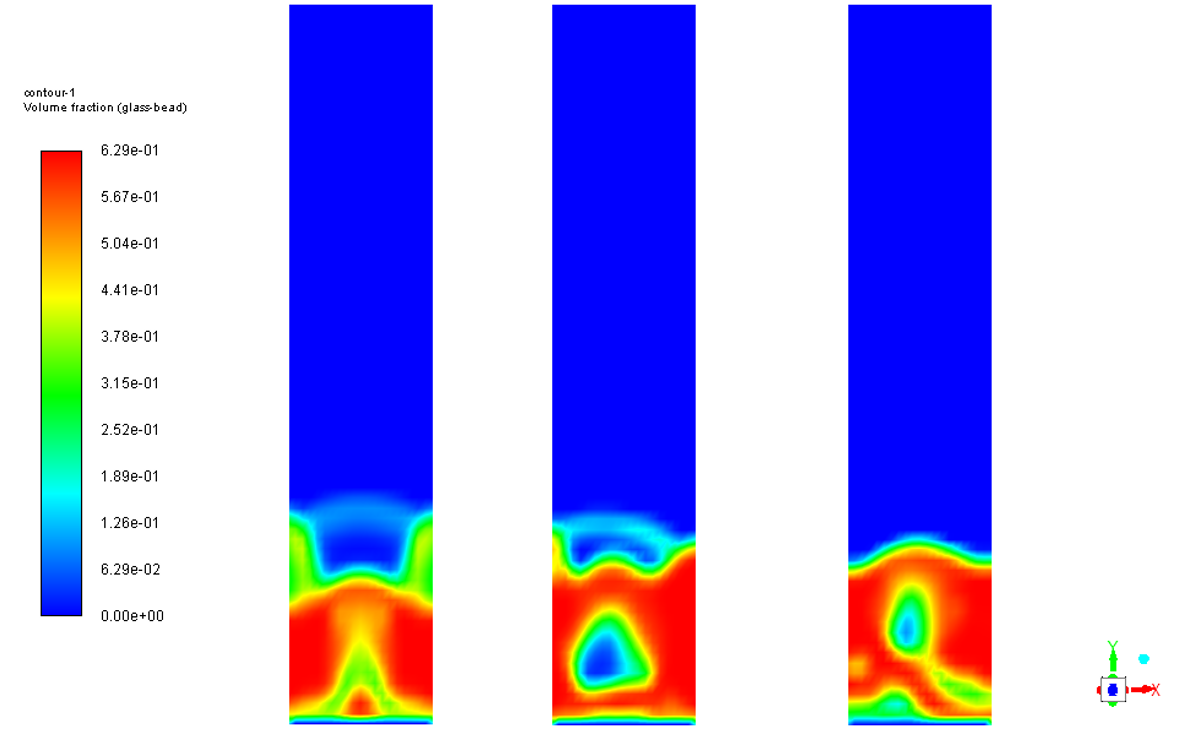
\includegraphics[width=0.48\linewidth]{volfrac_1_736.png}
    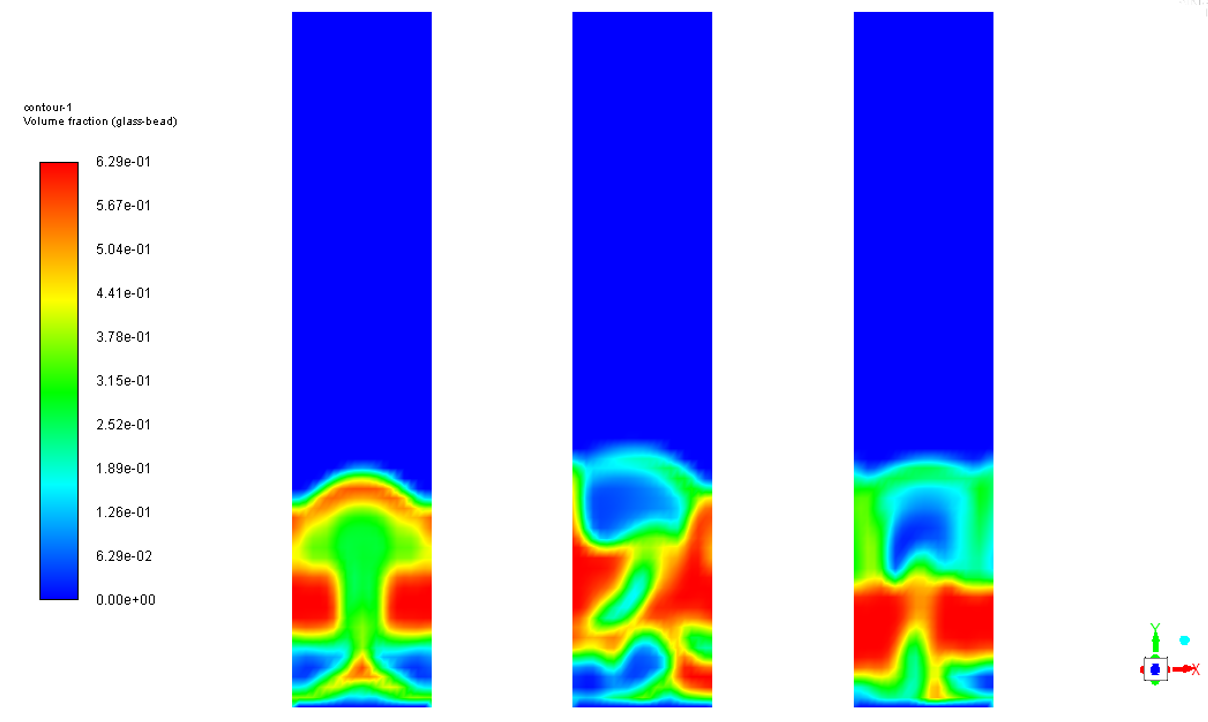
\includegraphics[width=0.48\linewidth]{volfrac_2_78.png}
    \caption{Solid Volume Fraction contours. Left: $1.736$ m/s. Right: $2.78$ m/s.}
\end{figure}

\begin{figure}[h!]
    \centering
    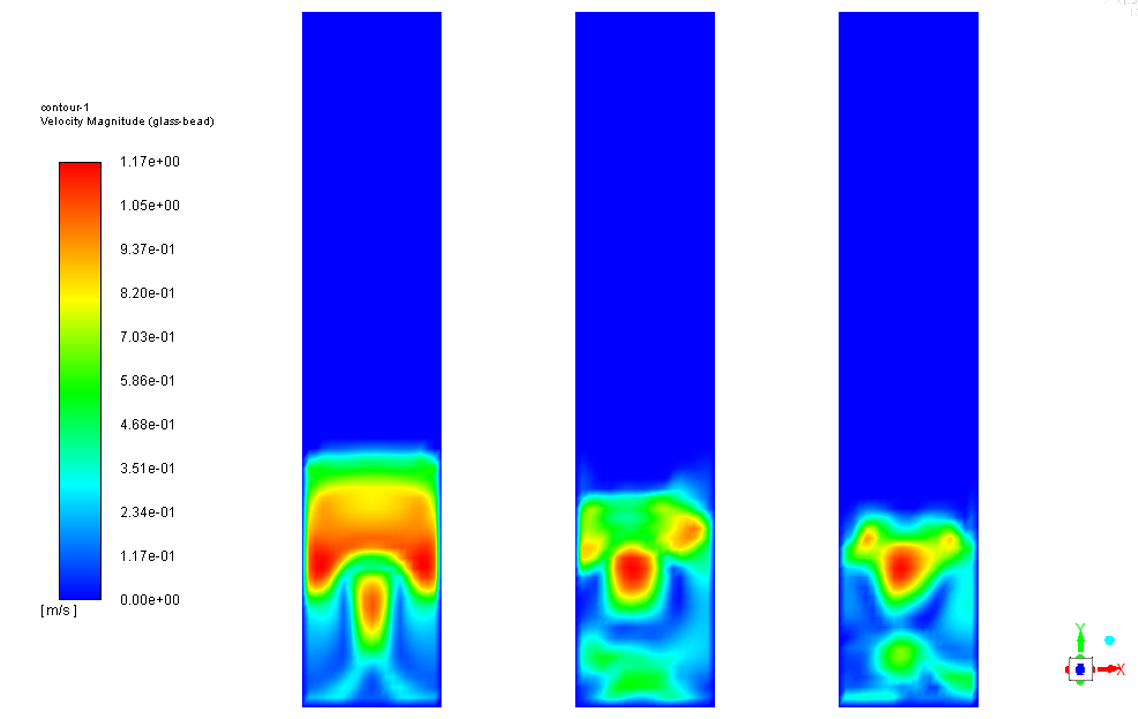
\includegraphics[width=0.48\linewidth]{velmag_1_736.png}
    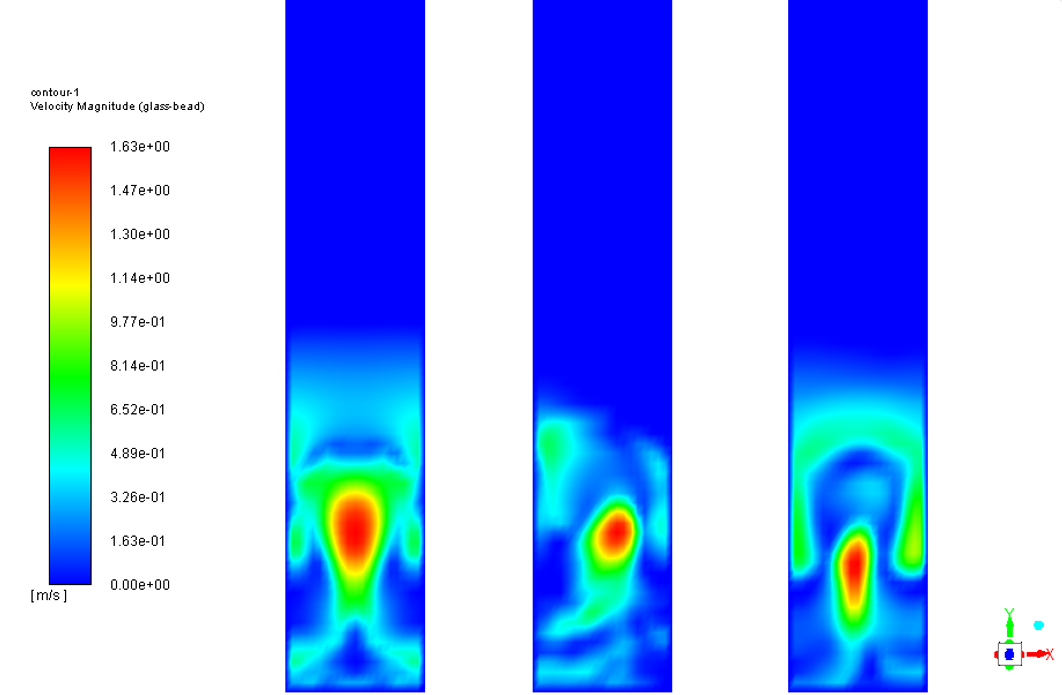
\includegraphics[width=0.48\linewidth]{velmag_2_78.png}
    \caption{Solid Velocity Magnitude contours. Left: $1.736$ m/s. Right: $2.78$ m/s.}
\end{figure}

\end{document}
